\section{Simulación de Enmascaramiento (o \textit{Masking})}
\label{sec:masking_dist_mask}
%Empezamos definiendo la simulación de masking. En \cite{DemasiCMA17}, se definió una simulación basada en estados para la masking-tolerancia a fallas, aquí reformulamos esta definición usando simulación basada en transiciones. Primero, vamos a introducir algunos conceptos que son necesarios para definir masking-tolerancia a fallas. Para todo vocabulario $\Sigma$, y todo conjunto de etiquetas $\Faults = \{F_0, \dots, F_n\}$ no pertenecientes a $\Sigma$, consideramos $\SigmaF = \Sigma \cup \Faults$, donde $\Faults \cap \Sigma = \emptyset$. 
La simulación de enmascaramiento provee una forma de verificar si una implementación tolerante a fallas es correcta al comprobar que un modelo que sirve de implementación (el cuál incluye fallas y mecanismos de tolerancia a fallas) se comporta como el modelo nominal (es decir, la especificación del sistema asumiendo que no hay fallas) siguiendo reglas del estilo de una bisimulación.
En \cite{DemasiCMA17}, se definió una simulación basada en estados para la tolerancia a fallas enmascarante, aquí reformulamos esta definición usando simulación basada en transiciones. 

Para todo vocabulario $\Sigma$, y todo conjunto de etiquetas $\Faults = \{F_0, \dots, F_n\}$ con $\Faults \cap \Sigma = \emptyset$, consideramos $\SigmaF = \Sigma \cup \Faults$. 
Intuitivamente, los elementos de $\Faults$ indican la ocurrencia de una falla en una implementación defectuosa. Además, a veces será útil considerar el conjunto $\Sigma^i = \{ e^i \mid e \in \Sigma\}$, que contiene los elementos de $\Sigma$ indexados con el superíndice $i$.

%, $\Sigma^i = \{\sigma^i \mid \sigma \in \Sigma\}$.

\subsection{Simulación de Enmascaramiento Fuerte}
\begin{definition} \label{def:masking_rel}
  Sean $A =\langle S, \Sigma, \rightarrow, s_0\rangle$ y $A' =\langle S', \SigmaF, \rightarrow', s_0' \rangle$ dos sistemas de transición etiquetados.
  $A'$ es \emph{fuertemente tolerante a fallas enmascarante} con respecto a $A$ si existe una relación 
$\M \subseteq S \times S'$ entre $A$ y $A'$ tal que:

\begin{enumerate}[(A)]
  \item $s_0 \M s'_0$, y
  \item para todo $s \in S, s' \in S'$ con $s \M s'$ y todo $e \in \Sigma$ vale lo siguiente:

  \begin{enumerate}[(1)]
    \item 
    si $s \xrightarrow{e} t$ entonces
    $\exists\; t' \in S': s' \xrightarrowprime{e} t'  \wedge t \M t'$;

      \item si $s' \xrightarrowprime{e} t'$ entonces
      $\exists \; t \in S: s \xrightarrow{e} t \wedge t \M t'$;

      \item si $s' \xrightarrowprime{F} t' $ para algún $F \in \Faults$ entonces
      $s \M t'$.
      
  \end{enumerate}
\end{enumerate}

Si tal relación existe, decimos que $A'$ es una \emph{implementación fuertemente tolerante a fallas enmascarante} de $A$, denotado como $A \Masking A'$. 
\end{definition}

Observemos que la definición es la estándar de bisimulación fuerte a excepción de que las etiquetas de fallas son tratadas de forma diferente ya que solo aparecen en el modelo de la implementación.  En este sentido, una falla producida por la implementación $A'$ es enmascarada apropiadamente si permanece desapercibida por el modelo nominal $A$ (ver regla (B.3)).
%
Más específicamente, la condición (A) establece que $A$ y $A'$ se relacionan en sus estados iniciales, y las condiciones (B.1) y (B.2) son las propiedades de transferencia típicas de bisimulaciones limitadas a el comportamiento nominal (es decir todas las transiciones que no están etiquetadas como fallas).
%
Sin embargo, la condición (B.3) establece que siempre que una falla se produzca en el modelo de la implementación $A'$, el modelo nominal $A$ solo puede imitar la acción quedándose en el mismo estado (es decir, haciendo nada).
%Intuitivamente, la definición establece que, partiendo de $s'$, las fallas pueden ser enmascaradas de tal forma que el comportamiento exhibido es el mismo que el observado al partir de $s$ ejecutando transiciones sin fallas. 
%En otras palabras, una relación de masking asegura que cualquier comportamiento defectuoso en la implementación puede ser simulado por la especificación. Mas específicamente, note que las condiciones (A), (B.1) y (B.2) implican que tenemos una bisimulación cuando $A$ y $A'$ no exhiben comportamientos defectuosos.
%Particularmente, la condición (B.1) dice que la ejecución normal de $A$ puede ser simulada por una ejecución de $A'$. Por otro lado, la condición (B.2) dice que la implementación no agrega más comportamientos normales (no defectuosos). Por ultimo, la condición (B.3) establece que toda transición defectuosa ($F$) que salga de $s'$ debe ser emparejada por un movimiento de $s$ a si mismo (es decir la especificación no hace nada).

\subsection{Simulación de Enmascaramiento Débil}

Para analizar sistemas menos triviales se necesita una relación de simulación de enmascaramiento débil. La idea principal es que una simulación de enmascaramiento débil se abstrae del comportamiento interno, el cual es modelado por una acción especial $\tau$. Observemos que las transiciones internas son comunes en tolerancia a fallas: las acciones ejecutadas como parte de un mecanismo tolerante a fallas en un componente usualmente no son observables para el resto del sistema.

Sea $A =\langle S, \Sigma \cup \{\tau\} \cup \Faults,  \rightarrow, s_0\rangle$ un sistema de transición etiquetado. Primero, consideremos la relación binaria ${\Rightarrow} \subseteq S \times S$ definida como la clausura reflexo-transitiva de $\xrightarrow{\tau}$, es decir, ${\Rightarrow} = {\xrightarrow{\tau}^*}$.  En otras palabras, decimos que $s \Rightarrow s'$ si hay un camino finito:  $s_0 \xrightarrow{\tau} s_2 \xrightarrow{\tau} \dots \xrightarrow{\tau} s_n$ tal que $s = s_0$, $s' = s_n$ y $n \geq 0$.
 %$\Sigma$ contains a distinguished \textit{silent} action $\tau$.
$\Rightarrow$ se puede extender a una relación etiquetada ${\Rightarrow} \subseteq S\times (\Sigma \cup \{\tau\} \cup \Faults) \times S$ de la siguiente manera: para todo $s,s'\in S$ y $e\in {\Sigma \cup \{\tau\} \cup \Faults}$,
 %for all $e \in \Sigma \cup \{\tau\}$ in such a way that $\Rightarrow$ (also denoted as $E_W$)  
 %is the relation $E$ preceded and followed by a arbitrary number of $\tau$ transitions. Formally:\\
 %
 \[
s \xRightarrow{e} s' \text{ \ ssi \ }
        \begin{cases}
            \exists t,t'\in S \colon s \Rightarrow t \xrightarrow{e} t' \Rightarrow s' & 
             \text{si } e \in \Sigma,  \\ 
            s \Rightarrow s' & \text{si } e = \tau,  \\
            s \xrightarrow{e} s' & \text{si } e \in \Faults.\\
        \end{cases}
 \]
 %
%The symbol $\circ$ stands for composition of binary relations.
 
 %

%Las \textit{relaciones de transición débiles} ${\Rightarrow} \subseteq S
%\times (\Sigma \cup \{\tau\} \cup \Faults) \times S$ consideran el paso \emph{silencioso} $\tau$ que se define como sigue: 

%\[
%\xRightarrow{e} = 
%       \begin{cases}
%            \xrightarrowstar{\tau} \circ \xrightarrow{e} \circ \xrightarrowstar{\tau} & 
%            \text{si } e \in \Sigma,  \\ 
%            \xrightarrowstar{e} & \text{si } e = \tau,  \\
%            \xrightarrow{e} & \text{si } e \in \Faults.\\
%       \end{cases}
%\]
%
%El símbolo $\circ$ representa la composición de relaciones binarias y $\xrightarrowstar{\tau}$ es la clausura reflexo-transitiva de la relación binaria $\xrightarrow{\tau}$. 

Intuitivamente, si $e \notin \{\tau\}\cup\Faults$, entonces $s\xRightarrow{e}s'$ significa que existe una secuencia de cero o mas transiciones $\tau$ empezando en $s$, seguido de una transición etiquetada por $e$, seguida luego por cero o mas transiciones $\tau$ eventualmente llegando a  $s'$.
$s \xRightarrow{\tau} s'$ establece que $s$ puede moverse a $s'$ por medio de cero o mas transiciones $\tau$.
%
En particular, $s \xRightarrow{\tau} s$ para todo $s$.
%
Para el caso en que $e\in\Faults$,
$s\xRightarrow{e}s'$ es equivalente a $s\xrightarrow{e}s'$ y por lo tanto no se permite ningún paso $\tau$ antes o después de la transición $e$.

\begin{definition} \label{def:weak_mask}
  Sean $A =\langle S, \Sigma, \rightarrow, \InitState \rangle$ y $A' =\langle S',
  \SigmaF, \rightarrow', \InitStatePrime \rangle$ dos sistemas de transición etiquetados con $\Sigma$
  conteniendo $\tau$ posiblemente.  $A'$ es \emph{débilmente tolerante a fallas enmascarante}
  con respecto a $A$ si existe una relación $\M \subseteq S
  \times S'$ entre $A$ y $A'$ tal que:

\begin{enumerate}[(A)]
  \item $\InitState \M \InitStatePrime$
  \item para todo $s \in S, s' \in S'$ con $s \M s'$ y todo $e \in \Sigma \cup \{\tau\}$ vale lo siguiente:

  \begin{enumerate}[(1)]
    \item si $s \xrightarrow{e} t$ entonces 
    $\exists\; t' \in S': s' \xRightarrowprime{e} t' 
    \wedge t \M t'$;

      \item si $s' \xrightarrowprime{e} t'$ entonces  
      $\exists \; t \in S: s \xRightarrow{e} t  
      \wedge t \M t'$;

      \item si $s' \xrightarrowprime{F} t'$ para algún $F \in \Faults$ entonces 
      $s \M t'$.
  \end{enumerate}
\end{enumerate}

%
Si tal relación existe, decimos que $A'$ es una \emph{implementación débilmente tolerante a fallas enmascarante} de
$A$, denotado por $A \WeakMasking A'$.
\end{definition}

El siguiente teorema conecta la simulación de enmascaramiento fuerte con la débil. El teorema establece que la simulación de enmascaramiento débil se vuelve una simulación de enmascaramiento fuerte cuando la transición $\xrightarrow{}$ es reemplazada por $\xRightarrow{}$ en la estructura original.

\begin{theorem} \label{thm:weak_thm}
  Sean
$A =\langle S, \Sigma, \rightarrow, \InitState \rangle$ y $A' =\langle S', \SigmaF, \rightarrow', \InitStatePrime \rangle$. 
$\M \subseteq S \times S'$ entre $A$ y $A'$ es una simulación de enmascaramiento débil si y solo si:

\begin{enumerate}[(A)]
  \item $\InitState \M \InitStatePrime$, y
  \item para todo $s \in S, s' \in S'$ con $s \M s'$ y todo $e \in \Sigma \cup \{\tau\}$ vale lo siguiente:

  \begin{enumerate}[(1)]
    \item si $s \xRightarrow{e} t$ entonces $\exists\; t' \in S': s' \xRightarrowprime{\text{e}} t' 
    \wedge t \M t'$;

      \item si $s' \xRightarrowprime{e} t'$ entonces 
      $\exists \; t \in S: s \xRightarrow{e} t \
      \wedge t \M t')$;

      \item si $s' \xRightarrowprime{F} t'$ para algún $F \in \Faults$ entonces 
      $s \M t'$
  \end{enumerate}
\end{enumerate}

\end{theorem}

\noindent
\begin{proof}
Primero observemos que las condiciones (A), (B.1), (B.2) y (B.3) de este teorema implican directamente a las condiciones (A), (B.1), (B.2) y (B.3) de la Definición~\ref{def:weak_mask}, respectivamente. Por lo tanto, la parte ``si'' de la prueba es directa. Para la parte ``solo si'', la condición (A) es la misma tanto en el teorema como en la definición.
Para la condición (B), tomamos $s \M s'$ y procedemos de la siguiente forma.

Para (B.1), asumamos que $s \xRightarrow{e} t$ para $e \in \Sigma \cup \{\tau\}$ y $t \in S$.
Procedemos por casos.

Si $e = \tau$, entonces, por definición de $\xRightarrow{\tau}$, existen $s_0,s_1,\ldots,s_n$ con $n\geq0$ tal que $s=s_0\xrightarrow{\tau}s_1\xrightarrow{\tau}{\cdots}\xrightarrow{\tau}s_n=t$.
%
Por la propiedad (B.1) de la Definición~\ref{def:weak_mask}, existen $s'_0,s'_1,\ldots,s'_n$ tal que $s'=s'_0\xRightarrowprime{\tau}s'_1\xRightarrowprime{\tau}{\cdots}\xRightarrowprime{\tau}s'_n$ y $s_i \M s'_i$ para $0<i\leq n$. Por lo tanto $s' \xRightarrowprime{\tau} t'$ y $t \M t'$ al tomar $t'=s'_n$.

Si $e \in \Sigma$, por definición de $\xRightarrow{\tau}$, existen $\hat{s}$ y $\hat{t}$ tal que $s\xRightarrow{\tau}\hat{s}\xrightarrow{e}\hat{t}\xRightarrow{\tau}t$.
Debido al caso previo para $\xRightarrow{\tau}$, y (B.1) de la Definición~\ref{def:weak_mask} para $\xRightarrow{e}$, existen $s'$, $\hat{s}'$, $\hat{t}'$ y $t'$ tal que $s'\xRightarrowprime{\tau}\hat{s}'\xRightarrowprime{e}\hat{t}'\xRightarrowprime{\tau}t'$ con $\hat{s} \M \hat{s}'$, $\hat{t} \M \hat{t}'$ y $t \M t'$.
Por lo tanto, $s'\xRightarrowprime{e}t'$ y $t \M t'$.

La condición (B.2) se deduce de forma similar.

Para (B.3), supongamos $s' \xRightarrowprime{F} t'$ para algún $t' \in S'$.  Entonces, por definición de ${\xRightarrowprime{F}}$, $s' \xrightarrowprime{F} t'$.  Utilizando la propiedad (B.3) de la Definición~\ref{def:weak_mask} se deduce que $s \M t'$, lo cual concluye la prueba.
%Primero observemos que las condiciones (A), (B.1), (B.2) y (B.3) en este teorema implican las condiciones (A), (B.1), (B.2) y (B.3)
% de la Definición~\ref{def:weak_mask}, entonces la parte ``si'' es directa. Para la otra dirección, la condición (A) es la misma en el teorema y en la definición.
% Supongamos ahora que la condición (B.1) de la Definición~\ref{def:weak_mask} vale, es decir,
% $s \xRightarrow{e} t$ para $e \in \Sigma \cup \{\tau\}$ y $t \in S$. 
%Si $e \in \Sigma$, entonces, por definición de$\Rightarrow$, tenemos que existen $w$ y $v$ tal que $s \xrightarrowstar{\tau} w$, $w \xrightarrow{e} v$
% y $v \xrightarrowstar{\tau} t$. Por lo tanto, por definición de $\Rightarrow$ y por la condición (B.2) de la Definición \ref{def:weak_mask} 
% tenemos que existen estados $s',t',w',v' \in S'$
% tales que $s' \xRightarrow{\tau} w'$, $w' \xRightarrow{e} v'$, y $v' \xRightarrow{\tau} t'$ y, 
% además, $w \M w'$, $v \M v'$, y $t \M t'$ lo cual implica que$s' \xRightarrow{e} t'$. 
% La prueba para la condición (B.2) es similar.
% 	Supongamos ahora que $s \M s'$ y $s' \xRightarrow{F} t'$, para algún $t' \in S'$. Entonces, por Definición de 
%$\Rightarrow$, tenemos que $s' \xrightarrow{F} t'$ y por Definición~\ref{def:weak_mask}
% tenemos $s \M t'$ . Esto concluye la prueba.
 \qedhere 
 \end{proof} 
 
Una forma natural de verificar bisimilitud débil es por medio de \emph{saturar}
el sistema de transición  \cite{FernandezM91,Milner89} y luego verificar bisimilitud fuerte sobre el sistema de transición saturado.
Similarmente, el Teorema~\ref{thm:weak_thm} nos permite computar simulación de enmascaramiento débil sobre $A =\langle S, \Sigma, \rightarrow, \InitState \rangle$ y $A' =\langle S', \SigmaF, \rightarrow', \InitStatePrime \rangle$ al reducir este problema al de computar simulación de enmascaramiento fuerte sobre las versiones saturadas $\textrm{sat}(A) =\langle S, \Sigma, \Rightarrow, \InitState \rangle$ y $\textrm{sat}(A') =\langle S', \SigmaF, \Rightarrow', \InitStatePrime \rangle$. 

En lo que resta del capítulo utilizaremos el Teorema~\ref{thm:weak_thm} para demostrar propiedades sobre enmascaramiento débil. Vale la pena destacar que la mayoría de las propiedades de enmascaramiento fuerte pueden ser también demostradas para enmascaramiento débil aplicando el Teorema~\ref{thm:weak_thm}.
	
\begin{example}
Consideremos el siguiente ejemplo, consideramos una celda de memoria que almacena un bit de información y soporta operaciones de lectura y escritura, presentado en forma basada en estados en \cite{DemasiCMA17}. Un estado en este sistema mantiene el valor corriente de la celda de memoria ($m=i$, para $i=0,1$), escribir le permite a uno cambiar este valor, y leer retorna el valor almacenado.  
Obviamente, en este sistema el resultado de una lectura va a depender del valor almacenado en la celda. 
Por lo tanto, una propiedad que uno podría asociar a este modelo es que el valor leído de la celda coincida con el de la ultima escritura que se haya ejecutado en el sistema.
    
Una falla que potencialmente se puede dar en este escenario ocurre cuando la celda inesperadamente pierde su carga, y su valor almacenado cambia (e.g., cambia de $1$ a $0$ debido a perdida de carga). Una técnica típica para lidiar con esta situación es \emph{redundancia}: usar tres bits de memoria en lugar de solo uno. Las operaciones de escritura se realizan simultáneamente sobre los tres bits. La lectura, por otro lado, retorna el valor que se repite en la mayoría de bits, esto se conoce como \emph{votación}. 

Adoptamos el siguiente enfoque para modelar este sistema. Las etiquetas $\text{w}_0, \text{w}_1, \text{r}_0,$ y $\text{r}_1$
representan las operaciones de escritura y lectura. Específicamente, $\text{w}_0$ (resp. $\text{w}_1$): escribe el valor cero (resp. uno) en la celda de memoria. $\text{r}_0$ (resp. $\text{r}_1$): lee el valor cero (resp. uno) almacenado en la celda de memoria.
La Figura~\ref{figure:exam_1_mem_cell} muestra tres sistemas de transición de estados. El primero de izquierda a derecha representa el sistema nominal para este ejemplo (denotado como $A$).
Tanto el segundo como el tercer sistema de transición son implementaciones tolerantes a fallas de $A$, denotados como $A'$ y $A''$ respectivamente. Observemos que $A'$ contiene una falla, mientras que $A''$ considera dos fallas. Ambas implementaciones usan redundancia triple; intuitivamente, el estado $\text{t}_0$ contiene tres bits con valor cero y $\text{t}_1$ contiene tres bits con valor uno.
Además, el estado $\text{t}_2$ se alcanza cuando uno de los bits cambió de valor (001, 010 o 100)
En  $A''$, el estado $\text{t}_3$ se alcanza después de que cambia un segundo bit (011, 101 o 110) empezando del estado $\text{t}_0$.
%\begin{figure}[h] 
%\begin{center}
%    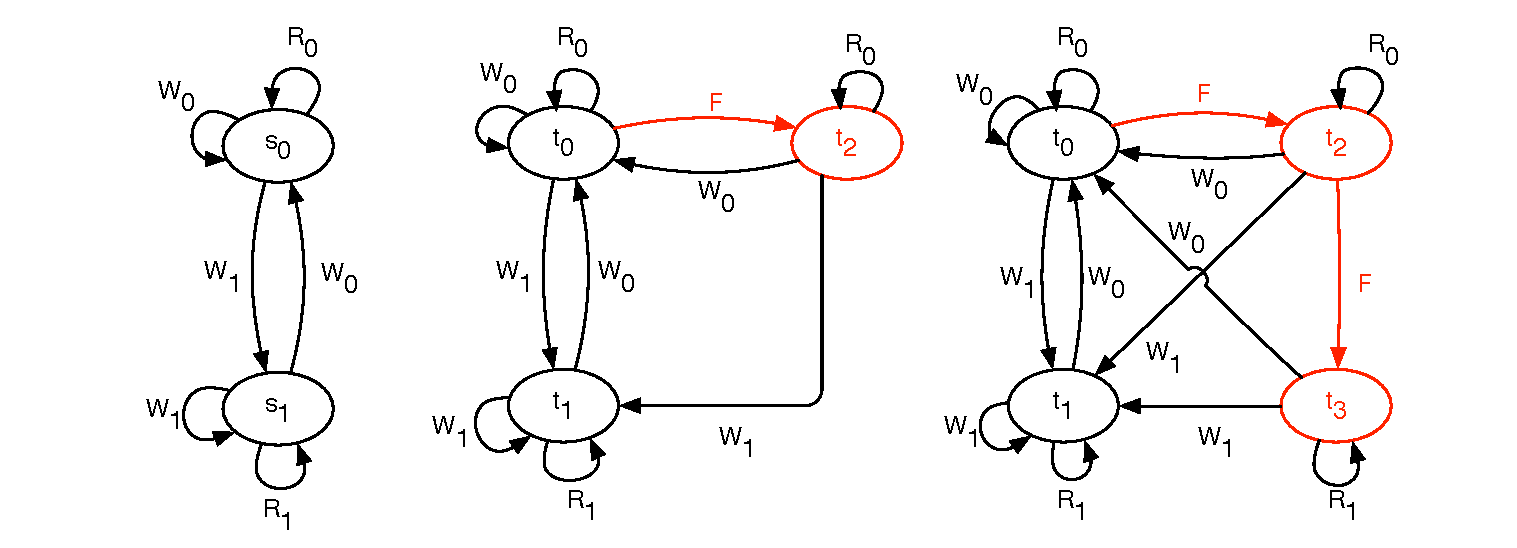
\includegraphics[scale=0.45]{Figs/example_1_cell_mem-eps-converted-to.pdf} 
   % \vspace{-1cm}
%    \caption{Modelo nominal y dos modelos con fallas de una celda de memoria.}
    %\vspace{-0.8cm}
%    \label{figure:exam_1_mem_cell}
%\end{center}
%\end{figure}
\begin{figure}[ht] 
\begin{center}
  % \includegraphics[scale=0.45]{example_1_cell_mem.eps} 
  % \vspace{-1cm}
  \begin{subfigure}{.26\textwidth}\centering
  \scalebox{1.1}{
  \begin{tikzpicture}[on grid,auto,align at top]
    \node[state] (n0)                   {$s_0$};
    \node[state] (n1) [below=2.3 of n0] {$s_1$};

    \path[-Latex]
    (n0) edge[bend right=15] node[swap] {$w_1$} (n1)
    (n0) edge[loop,out=60,in=120,looseness=5] node[above] {$w_0$} (n0)
    (n0) edge[loop,out=150,in=210,looseness=5] node[left] {$r_0$} (n0)
    (n1) edge[bend right=15] node[swap] {$w_0$} (n0)
    (n1) edge[loop,out=-60,in=-120,looseness=5] node[below] {$r_1$} (n1)
    (n1) edge[loop,out=150,in=210,looseness=5] node[left] {$w_1$} (n1)
    ;
  \end{tikzpicture}
  }
  \caption{Modelo nominal $A$}\label{figure:exam_1_mem_cell:nominal}
  \end{subfigure}
  %\hfill
  \begin{subfigure}{.32\textwidth}\centering
  \scalebox{1.1}{
  \begin{tikzpicture}[on grid,auto,align at top]
    \node[state] (n0)                   {$t_0$};
    \node[state] (n1) [below=2.3 of n0] {$t_1$};
    \node[state,red,fill=white,text=red] (n2) [right=2.3 of n0] {$t_2$};

    \path[-Latex]
    (n0) edge[red,bend left=15]  node {$F$}   (n2)
    (n0) edge[bend right=15] node[swap] {$w_1$} (n1)
    (n0) edge[loop,out=60,in=120,looseness=5] node[above] {$w_0$} (n0)
    (n0) edge[loop,out=150,in=210,looseness=5] node[left] {$r_0$} (n0)
    (n1) edge[bend right=15] node[swap] {$w_0$} (n0)
    (n1) edge[loop,out=-60,in=-120,looseness=5] node[below] {$r_1$} (n1)
    (n1) edge[loop,out=150,in=210,looseness=5] node[left] {$w_1$} (n1)
    (n2) edge[loop,out=60,in=120,looseness=5] node[above] {$r_0$} (n2)
    (n2) edge[bend left=15] node {$w_0$} (n0)
    (n2) edge[bend left=45] node {$w_1$} (n1)
    ;
  \end{tikzpicture}
  }
  \caption{Modelo con una falla $A'$}\label{figure:exam_1_mem_cell:onefault}
  \end{subfigure}
  %\hfill
  \begin{subfigure}{.32\textwidth}\centering
  \scalebox{1.1}{
  \begin{tikzpicture}[on grid,auto,align at top]
    \node[state] (n0)                   {$t_0$};
    \node[state] (n1) [below=2.3 of n0] {$t_1$};
    \node[state,red,fill=white,text=red] (n2) [right=2.3 of n0] {$t_2$};
    \node[state,red,fill=white,text=red] (n3) [below=2.3 of n2] {$t_3$};

    \path[-Latex]
    (n0) edge[red,bend left=15]  node {$F$}   (n2)
    (n0) edge[bend right=15] node[swap] {$w_1$} (n1)
    (n0) edge[loop,out=60,in=120,looseness=5] node[above] {$w_0$} (n0)
    (n0) edge[loop,out=150,in=210,looseness=5] node[left] {$r_0$} (n0)
    (n1) edge[bend right=15] node[swap] {$w_0$} (n0)
    (n1) edge[loop,out=-60,in=-120,looseness=5] node[below] {$r_1$} (n1)
    (n1) edge[loop,out=150,in=210,looseness=5] node[left] {$w_1$} (n1)
    (n2) edge[red]  node {$F$}   (n3)
    (n2) edge[loop,out=60,in=120,looseness=5] node[above] {$r_0$} (n2)
    (n2) edge[bend left=15] node {$w_0$} (n0)
    (n2) edge node[pos=0.25,inner sep=1pt] {$w_1$} (n1)
    (n3) edge node {$w_1$} (n1)
    (n3) edge[loop,out=-60,in=-120,looseness=5] node[below] {$r_1$} (n3)
    (n3) edge node[swap,pos=0.25,inner sep=1pt] {$w_0$} (n0)
    ;
  \end{tikzpicture}
  }
  \caption{Modelo con dos fallas $A''$}\label{figure:exam_1_mem_cell:twofaults}
  \end{subfigure}

  \caption{LTS para la celda de memoria.}
  %\vspace{-0.8cm}
  \label{figure:exam_1_mem_cell}
\end{center}
\end{figure}
\sloppy No es difícil ver que existe una relación de tolerancia a fallas enmascarante entre $A$ y $A'$, teniendo como testigo la relación $\M = \{(\text{s}_0, \text{t}_0), (\text{s}_1, \text{t}_1), (\text{s}_0, \text{t}_2)\}$. Es sencillo verificar que $\M$ satisface las condiciones de la Definición~\ref{def:masking_rel}.

Por otro lado, no existe una relación de enmascaramiento entre $A$ y $A''$ ya que el estado $\text{t}_3$ necesita estar relacionado con el estado $\text{s}_0$ en cualquier relación de enmascaramiento entre estos modelos. Este estado solo puede ser alcanzado con la ejecución de fallas, las cuales son necesariamente enmascaradas por transiciones ficticias. Sin embargo, observemos que, en el estado $\text{t}_3$, se puede leer el valor $1$ (la transición $\text{t}_3 \xrightarrow{\text{r}_1} \text{t}_3$) mientras que, en el estado $\text{s}_0$, solo se puede leer el valor $0$ (la transición $\text{s}_0 \xrightarrow{\text{r}_0} \text{s}_0$).
\end{example}
 
\subsection{Juego de Simulación de Enmascaramiento} \label{subsec:mask_sim_game}
Aquí procedemos a definir un juego de simulación de enmascaramiento para dos sistemas de transición de estados (la especificación del sistema nominal y su implementación tolerante a fallas) que captura la tolerancia a fallas enmascarante. Primero definimos el grafo de juego de enmascaramiento para dos jugadores, los cuales denominaremos como \emph{Refutador} ($\Refuter$) y \emph{Verificador}
($\Verifier$).

\begin{definition} \label{def:strong_masking_game_graph}
  Sean $A=\langle S, \Sigma, \rightarrow, \InitState \rangle$ y $A'=\langle S',
  \SigmaF, \rightarrow', \InitStatePrime \rangle$ dos sistemas de transición.
  % and $M \notin \Sigma \cup \SigmaF$.
  El \emph{grafo de juego de enmascaramiento fuerte} 
  $\StrMaskGG = \langle V^G, V_\Refuter, V_\Verifier, E^G, {\InitVertex}^G \rangle$ 
  para dos jugadores se define de la siguiente manera:

\begin{itemize}
    %\item $\Sigma^G = \Sigma^1 \cup \SigmaF^2$
  \item $V^G = (S \times ( \Sigma^1 \cup \SigmaF^2 \cup\{\#\}) \times S' \times \{ \Refuter, \Verifier \}) 
  \cup \{\ErrorSt\}$
  \item El estado inicial es $\InitVertex^G = \langle \InitState, \#, \InitStatePrime, \Refuter \rangle$, donde el Refutador comienza a jugar.
  \item Los estados del Refutador son $V_\Refuter = \{ (s, \#, s', \Refuter) \mid s \in S \wedge s' \in S' \} 
  \cup \{\ErrorSt\}$
  \item Los estados del Verificador son $V_\Verifier = \{ (s, \sigma, s', \Verifier) \mid s \in S \wedge s' \in S' \wedge \sigma \in ( \Sigma^1 \cup \SigmaF^2 )\}$
\end{itemize}
y $E^G$ es el conjunto mínimo que satisface que:
\begin{itemize}
  \item $\{ ( (s, \#, s', \Refuter) , (t, \sigma^{1}, s', \Verifier)) \mid \exists\;\sigma \in \Sigma: s \xrightarrow{\sigma} t \} \subseteq E^G$,

  \item $\{ ((s, \#, s', \Refuter), (s, \sigma^{2}, t', \Verifier))  \mid \exists\;\sigma \in \SigmaF: s' \xrightarrowprime{\sigma} t' \} \subseteq E^G$,

  \item $\{ ((s, \sigma^2, s', \Verifier), (t, \#, s', \Refuter)) \mid \exists\;\sigma \in \Sigma: s \xrightarrow{\sigma} t \} \subseteq E^G$,

  \item $\{ ((s, \sigma^1, s', \Verifier), (s, \#, t', \Refuter)) \mid \exists\;\sigma \in \Sigma: s' \xrightarrowprime{\sigma} t' \} \subseteq E^G$,

  \item $\{ ((s, F^2, s', \Verifier), (s, \#, s', \Refuter)) \} \subseteq E^G$, para cada $F \in \Faults$. 

  \item Si no hay transiciones que salgan de algún estado $v$, entonces, adicionalmente asumimos que $(v, \ErrorSt) \in E^G$ y $(\ErrorSt, \ErrorSt) \in E^G$.
\end{itemize}

\end{definition}

La intuición de este juego se detalla a continuación. 
El Refutador elige una transición de la especificación o de la implementación y hace su movimiento, luego el Verificador trata de igualar el movimiento de su contrincante en el modelo no elegido por el Refutador, esto es similar a un juego de bisimulación \cite{Stirling99}. 
Sin embargo, cuando el Refutador escoge una falla (solo este jugador puede elegir fallas), el Verificador debe igualar su movimiento con un movimiento ficticio (no se mueve en la especificación).
Esto intuitivamente se puede interpretar como un enmascaramiento de la falla por parte de la implementación tolerante a fallas de tal manera que la falla no puede ser observada del lado del usuario. El Refutador gana si el juego alcanza un estado de error, es decir, $\ErrorSt$; de lo contrario, el Verificador gana el juego. 
Básicamente este juego es un juego de alcanzabilidad \cite{Jurd11}.

Un \emph{grafo de juego de enmascaramiento débil} $\WeakMaskGG$ se define de la misma manera que su contraparte fuerte de la 
Definición~\ref{def:strong_masking_game_graph}, con la diferencia de que
$\Sigma$ y $\SigmaF$ pueden contener $\tau$, y que el conjunto de transiciones etiquetadas (denotado como $E_W^G$) ahora se define utilizando relaciones de transición débiles (es decir, $\Rightarrow$ y $\Rightarrow'$) de los sistemas de transición respectivos.

La Figura~\ref{figure:exam_2_mem_cell_gg_two_faults} muestra una parte del juego de enmascaramiento fuerte para el ejemplo que vimos considerando los sistemas de transición $A$ y $A''$. Aquí, los nodos del Refutador están representados gráficamente como cajas mientras que los nodos del Verificador están representados por círculos.
Podemos observar claramente en el grafo de juego que el Verificador no puede imitar la transición $((s_0, \#, t_3, R),(s_0, R_1^2, t_3, V))$
seleccionada por el Refutador, donde lee el valor $1$ en el estado $t_3$ de la implementación tolerante a fallas. Esto se da porque el Verificador solo puede leer el valor $0$ en el estado $s_0$. 
Entonces, el estado $\ErrorSt$ es alcanzado y el Refutador gana.

Como es de esperarse, hay una simulación de enmascaramiento fuerte entre $A$ y $A'$
si y solo si el Verificador tiene una estrategia ganadora en $\StrMaskGG$.

\begin{theorem} \label{thm:wingame_strat}
  Sean $A=\langle S, \Sigma, \rightarrow, \InitState \rangle$ y $A'=\langle S', \SigmaF, \rightarrow', \InitStatePrime \rangle$ dos sistemas de transición.
  Entonces, $A \Masking A'$ si y solo si el Verificador tiene una estrategia ganadora para el grafo de juego de enmascaramiento fuerte $\StrMaskGG$.
\end{theorem}

% PRUEBA PASADA AL APENDICE
\iffalse
\begin{proof} 
	``solo si'': Supongamos que existe una simulación de enmascaramiento $\M \subseteq S \times S'$.
La estrategia del Verificador (denominada $\pi^*$) se construye de la siguiente forma:  para los estados $(t, \sigma^1, s', V)$ (resp. $(s, \sigma^2, t', V)$) tal que el conjunto $\{ z' \in \post(s'): t \M z' \}$
(resp. $\{ z \in \post(s): z \M t' \}$) no es vacío y $\sigma \notin \Faults$, definimos $\pi^*(t, \sigma^1, s', \Verifier) = (t, \#, t', \Refuter)$ 
(resp. $\pi^*(s, \sigma^2, t', \Verifier) = (t, \#, t', \Refuter)$) que se corresponde con el arco $((t, \sigma^1, s', \Verifier), (t, \#, t', \Refuter))$ (resp. $((s, \sigma^2, t', \Verifier),(t, \#, t', \Refuter))$) tal que $t \in \{ z \in \post(s): z \M t' \}$ (resp. $t' \in \{ z' \in \post(s): z' \M t' \}$).  Si $\sigma \in \Faults$, entonces definimos $\pi^*(s, F^2, s', \Verifier) = (s, \#, s', \Refuter)$, para cualquier $F \in \Faults$, correspondiente con el arco $((s, F^2, s', \Verifier),( s, \#, s', \Refuter))$. Si el conjunto $\{ z' \in \post(s'): t \M z' \}$  (resp. $\{ z \in \post(s): z \M t' \}$) 
es vacío devuelve un vértice correspondiente a un arco arbitrario. 

	Probamos que cualquier jugada: $\rho_0 \rho_1 \dots$ (conforme a la estrategia $\pi^*$) cumple con: 
	(1) $\pr{3}{\rho_i}=\Verifier \vee \pr{0}{\rho_i} \Masking \pr{2}{\rho_i}$ y 
	(2) $\rho_i \neq \ErrorSt$, para todo $i\geq 0$. Esto implica que la estrategia es ganadora para el Verificador. 
La prueba es por inducción sobre $i$. El caso base es directo ya que 
$\InitVertex^G \neq \ErrorSt$ y $\InitVertex^G = (\InitState, \#, \InitStatePrime, \Refuter)$ y por suposición tenemos $\InitState \Masking \InitStatePrime$. Para el caso inductivo, asumimos que 
%\myworries{No entiendo esta frase}
%$\rho_i$ holds
$\rho_i \neq \ErrorSt$ y que $\pr{3}{\rho_i} = \Verifier$ o $\pr{0}{\rho_i} \Masking \pr{2}{\rho_i}$. 
Si $\rho_i = (s, \#, s', \Refuter)$, entonces esto significa que $s \Masking s'$. Como asumimos que
$\rightarrow$ y $\rightarrow'$ son seriales, tenemos que: $\exists \sigma \in \Sigma: s \xrightarrow{\sigma} t$ y $\exists \sigma \in \SigmaF : s' \xrightarrowprime{\sigma} t'$. Es decir, por definición del juego, $\rho_{i+1} \neq \ErrorSt$. 
Además, $\pr{3}{\rho_{i+1}} = \Verifier$ y entonces las aserciones (1) y (2) valen. 
Si $\rho_i = (s, \sigma^1, t, \Verifier)$ (resp. $\rho_i = (s, \sigma^2, t, \Verifier)$) y $\sigma \notin \Faults$,
tenemos que $\rho_{i-1} = (s, \#, s', \Refuter)$ y tenemos una transición $s \xrightarrow{\sigma} t$ (resp. $s' \xrightarrowprime{\sigma} t'$), por hipótesis inductiva, $s \Masking s'$. 
Por lo tanto, existe una transición $s' \xrightarrowprime{\sigma} t'$ (resp.  $s \xrightarrow{\sigma} t$) tal que $t \Masking t'$. 
La estrategia juega acorde a una de estas transiciones y entonces
$\rho_{i+1} = (t, \#, t', \Refuter)$ y $t \Masking t'$ y también $\rho_{i+1} \neq \ErrorSt$. Si $\sigma \in \Faults$, entonces $\rho_i = (s, F^2, t', \Verifier)$ para algún $F \in \Faults$. 
Por lo tanto, $\rho_{i-1} = (s, \#, s', \Refuter)$ con $s \Masking s'$ (por hipótesis inductiva). Esto significa que hay una transición $s' \xrightarrowprime{F} t'$, y por Definición~\ref{def:masking_rel},
tenemos que $s \Masking t'$. Además, por definición $\pi^*(s, F^2, t', \Verifier) = (s, \#,t',\Refuter)$, 
y además $s \Masking t'$. 

``si'': Supongamos que el Verificador tiene una estrategia ganadora (llamémosla $\pi$) 
desde el estado inicial. Entonces, definimos la relación de simulación de enmascaramiento de la siguiente manera: 
\[
\M = \{(s,s') \mid \Verifier \text{ tiene una estrategia ganadora para } (s, \#, s', \Refuter) \}.
\]
Vamos a probar que es una simulación de enmascaramiento. 
Primer, tenemos que $\InitState \M \InitStatePrime$ ya que $\pi$ es ganadora en $\InitVertex^G$. Por la condición (B.1) de la Definición~\ref{def:masking_rel}, si
$s \M s'$ y $s \xrightarrow{\sigma} t$ para algún $s \in S$ y $s' \in S'$, entonces debemos tener que $\pi$ es ganadora para cualquier estado $(s,\#,s',\Refuter)$. Además, por Definición~\ref{def:strong_masking_game_graph} existe un arco 
$((s,\#,s',\Refuter), (t,\sigma^1,s',\Verifier))$. 
Pero como $\pi$ es ganadora, también tenemos que $\pi(t,\sigma^1,s',\Verifier) \neq \ErrorSt$ y 
por lo tanto $\pi(t,\sigma^1,s',\Verifier)=(t, \#, t', \Refuter)$ y $\pi$ es ganadora desde  $(t, \#, t', \Refuter)$.
De este modo, hay una transición $t \xrightarrowprime{\sigma} t'$ tal que
$t \Masking t'$. La prueba para (B.2) es análoga. Para (B.3), asumamos que $s \Masking s'$ y $s' \xrightarrowprime{F} t'$ para algún 
$F \in \Faults$. 
Como antes, desde el estado $(s,\#,s',\Refuter)$, $\pi$ es ganadora donde también tenemos un arco $((s,\#,s',\Refuter), (s,F^2,t',\Verifier))$ por definición del juego. 
Como $\pi$ es ganadora desde $(s,\#,s',\Refuter)$ para el Verificador, existe una jugada $\pi(s,F^2,t',\Verifier) = (s,\#,t',\Refuter)$ tal que $\pi$ gana desde 
$(s,\#,t',\Refuter)$. Por lo tanto, $s \Masking t'$, y el resultado se deduce.
\qedhere

\end{proof} \\
\fi

Por el Teorema~\ref{thm:weak_thm}, el resultado también vale para juegos de enmascaramiento débiles, esto queda establecido en el siguiente teorema.

\begin{theorem} \label{thm:weak_wingame_strat}
  Sean $A=\langle S, \Sigma \cup \{\tau\}, \rightarrow, \InitState \rangle$ y
  $A'=\langle S', \SigmaF \cup \{\tau\}, \rightarrow', \InitStatePrime \rangle$.
  $A \WeakMasking A'$ si y solo si el Verificador tiene una estrategia ganadora para el grafo de juego de enmascaramiento débil $\WeakMaskGG$.
\end{theorem}

\begin{theorem}\label{thm:game-determined}
  Para cualquier $A$ y $A'$, el grafo de juego de enmascaramiento fuerte (resp.\ débil) 
  $\StrMaskGG$ (resp.\ $\WeakMaskGG$) puede ser determinado en tiempo $\BigO(|E^G|)$ (resp.\ $\BigO(|E_W^G|)$).
\end{theorem}
\begin{proof}
El conjunto de estados ganadores para el Refutador puede ser computado utilizando una búsqueda primero en ancho de abajo hacia arriba (\textit{bottom-up breadth-first search}) desde el estado de error, como en juegos de alcanzabilidad \cite{Jurd11}. 
Este procedimiento inspecciona cada arco, en el peor caso. Esto significa que el tiempo de ejecución de este algoritmo es $\BigO(|E^G|)$ para el caso de enmascaramiento fuerte, y $\BigO(|E_W^G|)$ para el caso débil. Para este ultimo caso, hay que tener en cuenta que computar  
$\Rightarrow$ a partir de $\rightarrow$ toma un tiempo polinomial.
\qedhere
\end{proof} \\
%\begin{figure} [ht]
%\begin{center}
    %\vspace{-0.5cm}
   % \includegraphics[scale=0.5]{ex1_cell_mem_game_graph_two_faults.eps} 
%    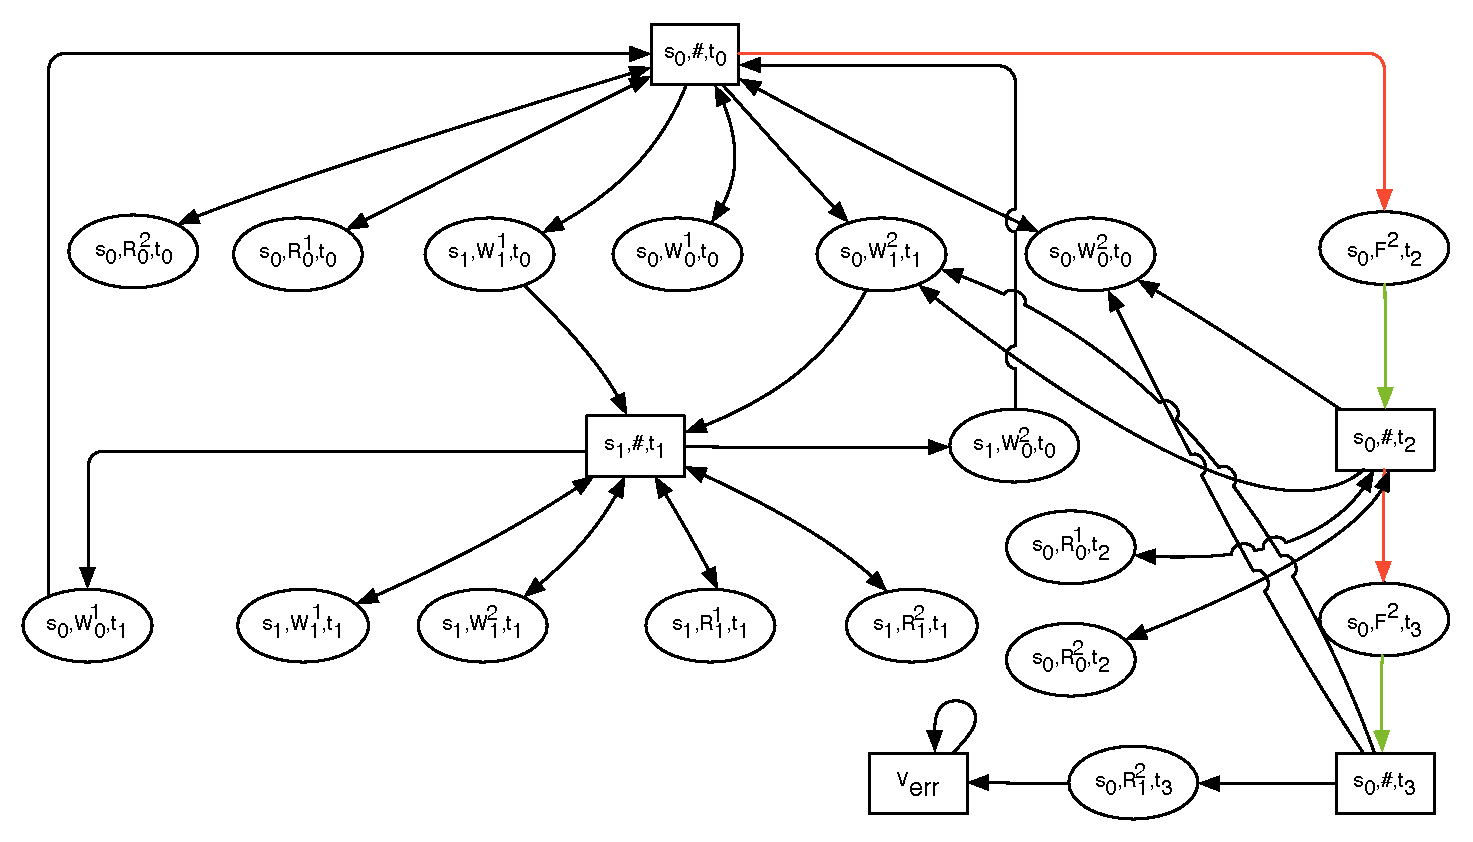
\includegraphics[scale=0.5]{Figs/ex1_cell_mem_game_graph_two_faults-eps-converted-to.pdf} 
  %  \vspace{-0.7cm}
%    \caption{Parte del grafo de juego de masking para la celda de memoria con dos fallas}
%    \label{figure:exam_2_mem_cell_gg_two_faults}
     %\vspace{-0.6cm}
%\end{center}
%\end{figure}

\begin{figure} [ht]
\begin{center}
  %% %\vspace{-0.5cm}
  %% % \includegraphics[scale=0.5]{ex1_cell_mem_game_graph_two_faults.eps} 
  %% \includegraphics[scale=0.5]{ex1_cell_mem_game_graph_two_faults.eps}
  %% %  \vspace{-0.7cm}

  \scalebox{0.8}{
  \begin{tikzpicture}[on grid,auto,align at top,
      hv path/.style={to path={-| (\tikztotarget)},rounded corners},
      vh path/.style={to path={|- (\tikztotarget)},rounded corners},
      hvh path/.style={to path={-- ++(#1,0) |- (\tikztotarget)},rounded corners}]
    
    \node[rvert] (s0xxxt0)                        {\makebox[4em][c]{$s_0,\#,t_0$}};

    \node[vvert] (s0w01t0) [below=2.2 of s0xxxt0] {\makebox[4em][c]{$s_0,w_0^1,t_0$}};
    \node[vvert] (s1w11t0) [left=2.0 of s0w01t0]  {\makebox[4em][c]{$s_1,w_1^1,t_0$}};
    \node[vvert] (s0r01t0) [left=2.0 of s1w11t0]  {\makebox[4em][c]{$s_0,r_0^1,t_0$}};
    \node[vvert] (s0r02t0) [left=2.0 of s0r01t0]  {\makebox[4em][c]{$s_0,r_0^2,t_0$}};
    \node[vvert] (s0w12t1) [right=2.0 of s0w01t0] {\makebox[4em][c]{$s_0,w_1^2,t_1$}};
    \node[vvert] (s0w02t0) [right=2.0 of s0w12t1] {\makebox[4em][c]{$s_0,w_0^2,t_0$}};
    \node[vvert] (s0ff2t2) [right=2.0 of s0w02t0] {\makebox[4em][c]{$s_0,F^2,t_2$}};

    \node[vvert] (s1w02t0) [below=2.2 of s0r02t0] {\makebox[4em][c]{$s_1,w_0^2,t_0$}};
    \node[rvert] (s1xxxt1) [below=2.2 of s1w11t0] {\makebox[4em][c]{$s_1,\#,t_1$}};
    \node[rvert] (s0xxxt2) [below=2.2 of s0ff2t2] {\makebox[4em][c]{$s_0,\#,t_2$}};

    \node[vvert] (s1w12t1) [below=2.2 of s1xxxt1] {\makebox[4em][c]{$s_1,w_1^2,t_1$}};
    \node[vvert] (s1w11t1) [left=2.0 of s1w12t1]  {\makebox[4em][c]{$s_1,w_1^1,t_1$}};
    \node[vvert] (s0w01t1) [left=2.0 of s1w11t1]  {\makebox[4em][c]{$s_0,w_0^1,t_1$}};
    \node[vvert] (s1r11t1) [right=2.0 of s1w12t1] {\makebox[4em][c]{$s_1,r_1^1,t_1$}};
    \node[vvert] (s1r12t1) [right=2.0 of s1r11t1] {\makebox[4em][c]{$s_1,r_1^2,t_1$}};
    \node[vvert] (s0r01t2) [right=2.0 of s0xxxt2] {\makebox[4em][c]{$s_0,r_0^1,t_2$}};

    \node[vvert] (s0ff2t3) [below=2.2 of s0xxxt2] {\makebox[4em][c]{$s_0,F^2,t_3$}};
    \node[vvert] (s0r02t2) [right=2.0 of s0ff2t3] {\makebox[4em][c]{$s_0,r_0^2,t_2$}};

    \node[rvert] (s0xxxt3) [below=2.2 of s0ff2t3] {\makebox[4em][c]{$s_0,\#,t_3$}};
    \node[vvert] (s0r12t3) [left=2.0 of s0xxxt3]  {\makebox[4em][c]{$s_0,r_1^2,t_3$}};
    \node[rvert] (verr)    [left=2.0 of s0r12t3]  {\makebox[4em][c]{$\ErrorSt$}};

    \path[{Latex[length=2.25mm,width=1.5mm]}-{Latex[length=2.25mm,width=1.5mm]},line width=0.7pt]
    (s0xxxt0) edge[bend right=15] (s0r02t0)
    (s0xxxt0) edge[bend right=10] (s0r01t0)
    (s0xxxt0) edge[]              (s0w01t0)
    (s0xxxt0) edge[bend left=10]  (s0w02t0)

    (s1xxxt1) edge[bend right=5]  (s1w11t1)
    (s1xxxt1) edge[]              (s1w12t1)
    (s1xxxt1) edge[bend left=5]   (s1r11t1)
    (s1xxxt1) edge[bend left=10]  (s1r12t1)
    (s0xxxt2) edge[]              (s0r01t2)
    (s0xxxt2) edge[]              (s0r02t2)
    ;

    \path[-{Latex[length=2.25mm,width=1.5mm]},line width=0.7pt]
    (s0xxxt0) edge[bend right=5]  (s1w11t0)
    (s0xxxt0) edge[bend left=5]   (s0w12t1)
    (s0xxxt0) edge[red,hv path]   (s0ff2t2)
    
    (s1w11t0) edge[]              (s1xxxt1)
    (s0w12t1) edge[bend left=10]  (s1xxxt1)
    (s0ff2t2) edge[darkgreen]     (s0xxxt2)

    (s1xxxt1) edge[bend right=10] (s0w01t1)
    (s1xxxt1) edge[]              (s1w02t0)
    (s1w02t0.west) edge[hvh path=-3mm]  ($(s0xxxt0.west) + (0,1mm)$)
    (s0xxxt2) edge[bend left=5]   (s0w02t0)
    (s0xxxt2) edge[bend left=10]  (s0w12t1)
    (s0xxxt2) edge[red]           (s0ff2t3)

    (s0w01t1.west) edge[hvh path=-5mm]  ($(s0xxxt0.west) + (0,2.5mm)$)
    (s0ff2t3) edge[darkgreen]     (s0xxxt3)

    (s0xxxt3) edge[bend left=15]  (s0w02t0)
    (s0xxxt3) edge[bend left=20]  (s0w12t1)
    (s0xxxt3) edge[]              (s0r12t3)
    (s0r12t3) edge[]              (verr)
    (verr)    edge[loop,out=195,in=165,looseness=7] (verr)
    ;

  \end{tikzpicture}
  }
    
  \caption{Parte del grafo de juego de enmascaramiento para la celda de memoria con dos fallas.}
  \label{figure:exam_2_mem_cell_gg_two_faults}
  %\vspace{-0.6cm}
\end{center}
\end{figure}

Los juegos de alcanzabilidad se pueden solucionar computando conjuntos $\text{Reach}_0$ (estados ganadores para el Refutador) como un punto fijo de conjuntos $\text{Reach}^i_0$  \cite{Jurd11}.
Estas ideas pueden ser adaptadas a nuestro contexto para tener en cuenta la cantidad de fallas. Esto sera útil en las próximas secciones, donde la cantidad de fallas es importante para razonar sobre la versión cuantitativa de los juegos de enmascaramiento.
\begin{definition}\label{def:U} Dado un grafo de juego de enmascaramiento fuerte $\StrMaskGG$, 
los conjuntos $\setsUs$ (para $i,j \geq 0$) se definen de la siguiente manera:
\begin{align*}
  U^0_i =& U^j_0 = \emptyset,  \label{def:of:Uji} \\
  U_1^1 =&  \{\ErrorSt\},
  \hspace{12.5cm} {}\notag
\end{align*}
\vspace{-0.97cm}
\begin{align*}
  U_{i+1}^{j+1} =&
    \{v' \mid v' \in V_\Refuter \wedge \post(v') \cap U_{i+1}^j \neq \emptyset\} \\
    &\textstyle\cup
    %\{v' \mid v' \in S_V \wedge post(v') \subseteq \bigcup_{j'\leq j} U_{i+1}^{j'} \wedge post(v') \cap U^j_{i+1} \neq \emptyset \wedge \pr{2}{v'} \notin \Faults \} \\
    %NOTE: above is the original condition of TACAS paper
    \{v' \mid v' \in V_\Verifier \wedge \post(v') \subseteq \bigcup_{i'\leq i+1, j' \leq j}U_{i'}^{j'} \\
    &\phantom{==}\wedge \post(v') \cap U^j_{i+1} \neq \emptyset \wedge \pr{1}{v'} \notin \Faults \} \\
    &\textstyle \cup
    \{v' \mid  v' \in V_\Verifier \wedge \post(v') \subseteq \bigcup_{i'\leq i, j' \leq j}U_{i'}^{j'} \\
    &\phantom{==}\wedge \post(v') \cap \setsUs \neq \emptyset \wedge \pr{1}{v'} \in \Faults \}
    \hspace{12.5cm} {}\notag
\end{align*}
Además, $U^k = \bigcup_{i \geq 0} U_i^k$ y $U = \bigcup_{k \geq 0} U^k$.
\end{definition}
Intuitivamente, el subíndice $i$ en $U^k_i$ indica que $\ErrorSt$ es alcanzado después de que hayan ocurrido a lo sumo $i-1$ fallas y $k$ pasos.
El siguiente lema se demuestra de forma directa utilizando técnicas estándar de juegos de alcanzabilidad \cite{AlfaroHK07}.
Notemos que estos conjuntos también pueden ser computados para juegos débiles de forma similar utilizando la relación $\Rightarrow$.
\begin{lemma} \label{lm:RefWinStrat} El Refutador tiene una estrategia ganadora en $\mathcal{G}_{A, A'}$ (o $\mathcal{G}^W_{A, A'}$) si y solo si $\InitVertex^G \in U^k$, para algún $k$.
\end{lemma}

% PRUEBA PASADA AL APENDICE
\iffalse
\begin{proof} 
``solo si'': La prueba utiliza resultados estándar de juegos de alcanzabilidad. Mas específicamente, considere el conjunto $V^G \setminus U$, este conjunto es una trampa para el Refutador, es decir, si $(s,\sigma, s', \Verifier) \in V^G \setminus U$, entonces existe un $v \in \post((s,\sigma, s', \Verifier))$ tal que 
$v \in V^G \setminus U$, sino
$(s,\sigma, s', \Verifier) \in U^k$ para algún $k$. Similarmente, si $(s,\#, s', R) \in V^G \setminus U$, entonces para todo $v \in \post((s,\#, s', \Refuter))$ 
tenemos $v \in V^G \setminus U$. Esto significa que $V^G \setminus U$ es una ``trampa'' para el Refutador. 
Ahora bien, podemos definir una estrategia para el Verificador $\pi_\Verifier$ de la siguiente manera: si $(s, \sigma, s', \Verifier) \in V^G \setminus U$, entonces
$\pi_\Verifier(s, \sigma, s', \Verifier) = \rho$ para algún $v \in V^G \setminus U$ el (cuya existencia esta garantizada), de lo contrario retorna un nodo arbitrario. 
Esta estrategia es ganadora para el Verificador desde cualquier $v \in V^G$, es decir, para cualquier jugada $\rho_0 \rho_1 \rho_2 \dots$ 
si $\rho_0 \in V^G \setminus U$, entonces $\forall i \geq 0: \rho_i \in V^G \setminus U$ 
(lo cual implica que $\forall i \geq 0: \rho_i \neq \ErrorSt$). 
La prueba es por inducción sobre $i$. Para $i=0$ el resultado es directo ya que $\rho_0 \in V^G \setminus \{\ErrorSt\}$. Para el caso inductivo,
supongamos que $\rho_i \in V^G \setminus U$. En el caso de que $\rho_i = (s, \sigma, s', \Verifier)$, entonces por definición de $\pi_\Verifier$, 
$\rho_{i+1} = \pi_\Verifier(s,\sigma, s', \Verifier) \in V^G \setminus U$.
Además, si $\rho_i = (s, \#, s', \Refuter)$, entonces $\post((s, \#, s', \Refuter)) \subseteq V^G \setminus U$, 
y por lo tanto $\rho_{i+1} \notin U$. 
Ahora bien, como $\InitVertex^G \notin U^k$ para todo $k$, entonces $\InitVertex^G \notin U$ y $\InitVertex^G \in V^G \setminus U$. 
En consecuencia, por la propiedad demostrada arriba $\Refuter$ tiene una estrategia ganadora desde 
$\InitVertex^G$. Pero esto es una contradicción porque el Refutador y el Verificador no pueden tener ambos estrategias ganadoras desde los mismos estados.
Por consiguiente, $\InitVertex^G \in U^k$ para algún $k$.
	
``si'': Considere $\InitVertex^G \in U^k$ para algún $k$, es decir, tenemos  $\InitVertex^G \in U^k_i$ para algún $i$ por Definición~\ref{def:U}. 
Además, para cada $v \in V^G$ definimos $\delta(v) = \min \{ (i,j) \mid v \in U^j_i \}$ (usando orden lexicográfico), por conveniencia asumimos $\min \emptyset = (\infty, \infty)$.
Entonces, la estrategia ganadora $\pi_R$ para el Refutador se define de la siguiente forma. Si $\delta(v) = (i,j)$ (con $(i,j) < (\infty, \infty)$), entonces $\pi_\Verifier(v) = w$, con $w$ siendo un vértice tal que
$\delta(w) = (i,j-1)$ (si $\pr{1}{v} \notin \Faults$) o $\delta(w) = (i-1,j-1)$ (si $\pr{1}{v} \in \Faults$), cuya existencia esta garantizada por Definición~\ref{def:U}. De otra forma, $\pi_\Refuter(v)$ retorna
un vértice arbitrario. Note que para cualquier jugada $\rho_0 \rho_1 \rho_2 \dots$ comenzando en $\InitVertex^G$ tenemos que:  para todo $i \geq 0$, $\delta(\rho_i) > \delta(\rho_{i+1})$, en orden lexicográfico.
Por lo tanto, para algún $k>0$ tenemos $\delta(\rho_k) = (1,1)$, y por tanto $\rho_k = \ErrorSt$.
\qedhere
\end{proof} \\
\fi

Por el Teorema \ref{thm:weak_thm}, esta prueba también aplica al juego de enmascaramiento débil $\WeakMaskGG$.
%By theorem \ref{thm:weak_thm}, the proof also applies for the weak masking game graph $\mathcal{G}^W_{A, A'}$. 